\documentclass[10pt]{article}

% Manuscript v4 (draft, 17 Nov 2026), formatted after the ICLR conference style
% (single column, author-year citations, theorem environments). It is NOT under
% review anywhere. Every number comes from a saved run (Appendix C). Items marked
% \pending{...} have not been run and must be filled or removed before submission.
\usepackage[letterpaper,margin=1in]{geometry}
\usepackage{times}
\usepackage{amsmath,amssymb,amsthm}
\usepackage{booktabs}
\usepackage{graphicx}
\usepackage{array}
\usepackage{xcolor}
\usepackage{float}
\usepackage{algpseudocode}
\usepackage[round]{natbib}
\usepackage{hyperref}
\hypersetup{colorlinks=true,linkcolor=blue,citecolor=blue,urlcolor=blue}
\emergencystretch=2em

\newfloat{algorithm}{tbp}{loa}
\floatname{algorithm}{Algorithm}

\theoremstyle{plain}
\newtheorem{proposition}{Proposition}
\newtheorem{lemma}{Lemma}
\newtheorem{theorem}{Theorem}
\newtheorem{corollary}{Corollary}
\theoremstyle{definition}
\newtheorem{definition}{Definition}
\newtheorem{assumption}{Assumption}
\theoremstyle{remark}
\newtheorem{remark}{Remark}

\newcommand{\care}{\textsc{CARE}}
\newcommand{\evolve}{\textsc{ASEM-Evolve}}
\newcommand{\pending}[1]{\textcolor{red}{\textbf{[PENDING: #1]}}}
\newcommand{\sub}{\sqsubseteq}
\newcommand{\A}{\mathcal{A}}
\newcommand{\D}{\mathcal{D}}
\newcommand{\G}{\mathcal{G}}
\newcommand{\Rset}{\mathcal{R}}
\newcommand{\F}{\mathcal{F}}

\title{\textbf{Guarded Memory Graphs for Long-Horizon Conversational QA:\\
When a Second Read Helps, and What to Store Instead}}
\author{Anonymous authors\\ \small Draft v4 --- not under review}
\date{}

\begin{document}
\maketitle

\begin{abstract}
Agents that converse over months must answer questions whose evidence is
scattered, updated and attributed to different speakers. We study this problem
through a two-layer memory graph: an append-only archive of original turns that
is the only citable evidence, and a derived layer of versioned attribute notes
and typed edges that may evolve. Writes to the derived layer pass deterministic
guards; we prove that the guards preserve string-level grounding, a total order
of versions per attribute, and replayability from the archive. Reading is
retrieval-augmented: hybrid dense--lexical seeds, optional personalized-PageRank
expansion with a proven locality bound, and a bounded reader that may repair its
answer once. We then ask when that repair should be accepted and prove an exact
break-even condition and a rate condition for any acceptance verifier. Empirically,
with open models only (Qwen3-8B reader, Qwen3-Embedding-0.6B encoder), repair raises
the LoCoMo aggregate from 0.4588 to 0.5256 but reverses 46 correct refusals, and
raises a diagnostic LongMemEval F1 from 0.348 to 0.374 while correct abstentions
fall from 21/30 to 16/30. The rate condition requires a verifier to catch losses at
least 3.89 times as often as it rejects gains on LoCoMo; a same-model yes/no
verifier reaches 1.52 and, as predicted, lowers the repair gain from +133.1 to
+125.1 points. A pre-registered quote-grounded verifier in thinking mode catches
35 of 46 unsupported repairs but rejects half of the useful ones (ratio 1.53), and
also fails; all six verifier configurations we scored stay below the threshold and
all lower the gain, as the theory predicts. The 0.6B encoder recovers more annotated evidence than BM25
(recall at eight turns 0.617 versus 0.539 on LoCoMo, and higher in all ten
conversations), reversing an earlier conclusion drawn with MiniLM. End to end with
the same reader, it beats BM25 on the first read ($+0.014$, 9 of 10 conversations)
but not after repair ($-0.009$, interval including zero): answerable F1 is equal and
the remaining gap is abstention. Finally, on
multi-session questions, more recall does not yield more correct answers, which
motivates storing aggregable notes rather than re-reading. The write-path
evolution experiments are pre-registered but not yet run.
\end{abstract}

\section{Introduction}
\label{sec:intro}

Long-horizon conversational question answering stresses two capabilities at
once. The agent must \emph{access} evidence that has fallen outside its context
window, and it must \emph{combine} evidence that is spread over sessions, has been
superseded, or concerns a different speaker. Write-time memory systems organize
what is stored \citep{packer2023memgpt,chhikara2025mem0,amem2025,memoryr12025,cao2026higmem};
read-time systems keep the history and decide per question what to read
\citep{du2026memr3,wang2026cuemem,liu2026livectx,chen2026justmem,yu2026lazymem};
corrective retrieval-augmented generation retrieves again when the first attempt
looks insufficient \citep{jiang2023active,asai2023selfrag,yan2024crag}.

Two questions are rarely made precise. \emph{Which properties of a memory can be
guaranteed when the memory is allowed to change?} And \emph{when should a second
read override the first answer?} We address both with a formal model and test its
predictions on two benchmarks.

\paragraph{Contributions.}
\begin{enumerate}
  \item \textbf{A guarded memory graph} (Section~\ref{sec:graph}). We formalize memory as a typed
  multigraph over an immutable archive and a versioned derived layer, define
  write operators with code-checked guards, and prove grounding, version-chain
  and replayability invariants (Propositions~\ref{prop:grounding}--\ref{prop:replay}).
  \item \textbf{Graph RAG with bounded repair} (Section~\ref{sec:read}). Reading combines dense
  and lexical seeds by reciprocal-rank fusion, optional typed personalized
  PageRank with a locality bound (Lemma~\ref{lem:ppr}), archive projection of
  every cited node (Proposition~\ref{prop:projection}), and a repair policy with at most two
  reader calls (Proposition~\ref{prop:cost}).
  \item \textbf{A theory of repair acceptance} (Section~\ref{sec:accept}). We give an exact
  break-even identity (Theorem~\ref{thm:breakeven}) and a rate condition under an
  independence assumption (Corollary~\ref{cor:rate}), and show that the condition
  predicts the measured failure of a yes/no verifier.
  \item \textbf{Measurements with open models} (Section~\ref{sec:experiments}). The repair trade-off on
  LoCoMo and LongMemEval, the reversal of sparse-versus-dense retrieval with a
  current open encoder, a nine-system end-to-end comparison with a shared reader
  showing that the retriever and the repair step interact, and evidence that the
  residual error is aggregation rather than access.
\end{enumerate}

\begin{figure}[t]
\centering
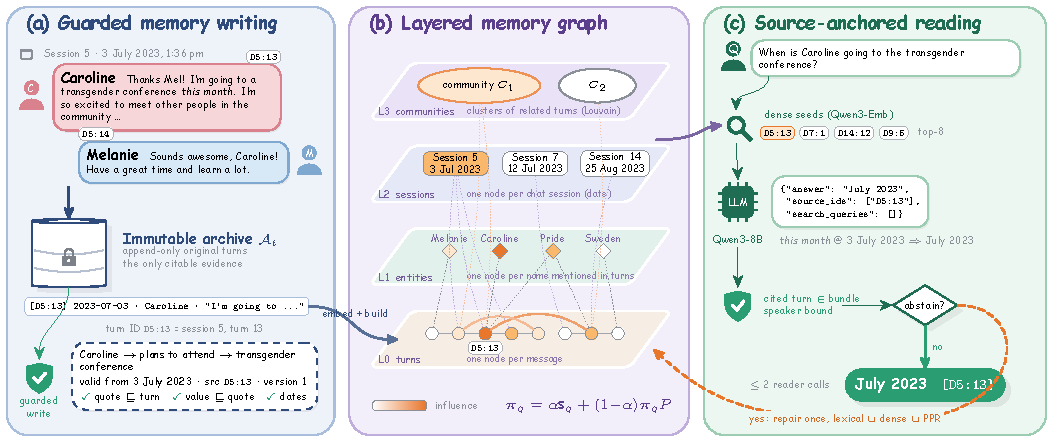
\includegraphics[width=\linewidth]{figures/asem_method_figure.pdf}
\caption{Overview. \textbf{(a)} Original turns enter an append-only archive, the only citable
evidence; guarded operators write versioned notes whose values must be quoted from a turn
(dashed: implemented and unit-tested, not yet evaluated end to end). \textbf{(b)} A four-layer
memory graph is built per conversation without an LLM; a question's personalized-PageRank mass
gives each node its influence. \textbf{(c)} The reader answers from a top-8 first bundle with
cited source IDs, code checks bind the citations to the bundle, and an abstention with
missing-evidence searches triggers at most one graph-aware repair. The example is real
(LoCoMo \texttt{conv-26}, question 17): the turns, the dense top-4 seeds and the reader's
answer \emph{July 2023} citing \texttt{D5:13} are the saved outputs of our run, with no repair
needed. Node shading and community memberships in (b) illustrate the mechanism and are not
computed values for this question.}
\label{fig:overview}
\end{figure}

\paragraph{Scope.} Contributions 1--3 are formal results; their empirical
counterparts are reported where they exist. The graph expansion of
Section~\ref{sec:ppr} and the aggregation operator of Section~\ref{sec:agg} are specified but
not yet evaluated, and we do not claim that memory evolution improves accuracy.

\section{Related Work}
\label{sec:related}

\paragraph{Persistent and evolving memory.}
MemGPT pages information between context and storage \citep{packer2023memgpt};
Mem0 extracts and consolidates facts \citep{chhikara2025mem0}; A-Mem links and
revises notes \citep{amem2025}; Memory-R1 learns write operations with
reinforcement learning \citep{memoryr12025}. HiGMem maintains an event--turn
hierarchy whose summaries are refreshed as turns arrive \citep{cao2026higmem}.
These systems evolve what is stored, but their update rules are learned or
prompted rather than guarded by checkable invariants, and none keeps a separate
immutable layer as the sole citation source.

\paragraph{Read-time access.}
MemR$^3$ routes among retrieval, reflection and answering while tracking evidence
gaps \citep{du2026memr3}; CueMem and LiveCtx rebuild query-specific context from
raw turns \citep{wang2026cuemem,liu2026livectx}. JustMem writes atomic cards once
per session and selects lookup, composition or source replay per query
\citep{chen2026justmem}. LazyMem defers construction to query time with a 4B
keep/drop model trained by GRPO \citep{yu2026lazymem}.

\paragraph{Graph retrieval.}
Personalized PageRank (PPR) gives local, seed-centred relevance on graphs
\citep{andersen2006local}; HippoRAG uses PPR over an entity graph for long-term
memory in retrieval-augmented generation \citep{gutierrez2024hipporag}. We use
typed PPR as an optional expansion over the derived layer and prove that it stays
local and citable.

\paragraph{Corrective retrieval.}
FLARE \citep{jiang2023active}, Self-RAG \citep{asai2023selfrag}, Adaptive-RAG
\citep{jeong2024adaptive} and CRAG \citep{yan2024crag} decide when to retrieve
again or how to correct retrieved evidence. Our acceptance theory concerns the
decision they all face after a second retrieval: whether to keep its answer.

\section{Problem Setting}
\label{sec:setting}

\paragraph{Conversation stream.}
A conversation is a stream of turns $s_i=(\mathrm{id}_i,\sigma_i,t_i,p_i,x_i)$
with session $\sigma_i$, session date $t_i$, speaker $p_i$ and text $x_i$. The
archive at time $t$ is $\A_t=\{s_i : i\le t\}$. For strings we write $u\sub w$
when $u$ is a contiguous substring of $w$.

\paragraph{Questions and scores.}
A question $q$ arrives at time $t_q$ and has a reference $y_q$, or is
\emph{unsupported} (its premise is not established by the conversation), in
which case the correct output is the abstention $\bot$. A system returns
$a\in\mathcal{Y}\cup\{\bot\}$ with citations $C\subseteq\A_{t_q}$ and earns a score
$m(a,y_q)\in[0,1]$; for unsupported questions $m=\mathbf{1}[a=\bot]$.

\paragraph{Memory state.}
The memory is $M_t=(\A_t,\D_t)$, where $\D_t$ is a derived layer defined in
Section~\ref{sec:graph}. The reader is a frozen language model; all adaptation is in $\D_t$
and in non-parametric scores.

\paragraph{Objective.}
For a question set $\mathcal{Q}$, maximize $\frac{1}{|\mathcal{Q}|}\sum_{q}m(a_q,y_q)$
subject to (i) every non-abstaining answer citing archive turns only, (ii) at most
two reader calls per question, and (iii) a serialized evidence budget of $L$
characters per call.

\section{The Guarded Memory Graph}
\label{sec:graph}

\subsection{Structure}

\begin{definition}[Memory graph]
\label{def:graph}
The memory graph at time $t$ is a typed multigraph $\G_t=(V_t,E_t,\psi)$ with
$V_t=\A_t\cup N_t$, where $N_t$ are note nodes, and edge types
$\psi:E_t\to\Rset$,
\[
\Rset=\{\textsf{next},\ \textsf{session},\ \textsf{cite},\ \textsf{supersede},\ \textsf{temporal},\ \textsf{entity},\ \textsf{causal}\}.
\]
\textsf{next} and \textsf{session} edges connect archive turns; \textsf{cite} edges
connect a note to its source turns; the remaining types connect notes.
\end{definition}

\begin{definition}[Note]
\label{def:note}
A note is $n=(k,v,\mathrm{Src}(n),\tau(n),\mathrm{ver}(n),\mathrm{st}(n))$ with key
$k=(\text{subject},\text{attribute})$, value $v$, source turns
$\mathrm{Src}(n)\subseteq\A_t$, validity time $\tau(n)$ equal to the date of its
source turn, version number $\mathrm{ver}(n)\in\mathbb{N}$ and status
$\mathrm{st}(n)\in\{\textsf{current},\textsf{superseded}\}$. The derived layer is
$\D_t=(N_t,E_t^{N})$, the notes with their note--note and \textsf{cite} edges.
\end{definition}

\begin{definition}[Grounding]
\label{def:grounded}
A note $n$ is \emph{grounded} in $\A_t$ if there are $s\in\mathrm{Src}(n)$ and a
quote $w$ with $w\sub x_s$ and $v\sub w$.
\end{definition}

Grounding is a string-level property: it rules out invented values, not wrong
interpretations. Assumption~\ref{ass:semantic} below makes the gap explicit.

\subsection{Guarded operators}

Each operator $O$ is a partial map $(\A_t,\D_t)\rightharpoonup(\A_t,\D_t')$
defined only where its guard $g_O$ holds; otherwise the state is unchanged and
the attempt is logged. Let $\mathrm{cur}_t(k)$ denote the set of current notes
with key $k$.

\begin{itemize}
  \item $\textsc{Add}(k,v,s,w)$: guard $s\in\A_t \land w\sub x_s \land v\sub w \land
  \mathrm{cur}_t(k)=\varnothing$. Effect: insert a current note of version 1 with
  $\tau=t_s$ and a \textsf{cite} edge to $s$.
  \item $\textsc{Update}(k,v,s,w)$: guard $s\in\A_t \land w\sub x_s \land v\sub w \land
  \mathrm{cur}_t(k)=\{n\} \land t_s\ge\tau(n) \land v\neq v(n)$. Effect: set
  $\mathrm{st}(n)\leftarrow\textsf{superseded}$, insert a current note $n'$ with
  $\mathrm{ver}(n')=\mathrm{ver}(n)+1$, $\tau(n')=t_s$, and a
  \textsf{supersede} edge $n\to n'$.
  \item $\textsc{Link}(n_1,n_2,r)$: guard $r\in\{\textsf{temporal},\textsf{entity},\textsf{causal}\}
  \land n_1\ne n_2 \land n_1,n_2\in N_t \land
  (\sigma(\mathrm{Src}(n_1))\cap\sigma(\mathrm{Src}(n_2))\neq\varnothing \lor
  \mathrm{Src}(n_1)\cap\mathrm{Src}(n_2)\ne\varnothing)$. Effect: add an
  undirected edge of type $r$.
  \item \textsc{Split}, \textsc{Merge}, \textsc{Prune}, \textsc{Reorg}: specified
  in Appendix~\ref{app:ops}; not covered by the propositions below.
\end{itemize}

The archive changes only by appending turns: $\A_{t+1}=\A_t\cup\{s_{t+1}\}$, and
no operator modifies $x_s$ for any $s$.

\begin{algorithm}[t]
\caption{Guarded write step after a new session (\evolve{})}
\label{alg:write}
\begin{algorithmic}[1]
\Require archive $\A$, derived layer $\D$, new turns $S$, extractor $X$
\State $\A\gets\A\cup S$ \Comment{append only}
\For{each proposal $(\text{op},k,v,s,w)\in X(S,\D)$}
  \If{$g_{\text{op}}(k,v,s,w;\A,\D)$}
    \State $\D\gets \text{op}(\D)$; \ \textsc{Log}(op, applied)
  \Else
    \State \textsc{Log}(op, rejected, reason)
  \EndIf
\EndFor
\State \Return $\A,\D$
\end{algorithmic}
\end{algorithm}

\subsection{Invariants}

\begin{assumption}[Append-only archive]
\label{ass:archive}
For all $t\le t'$, $\A_t\subseteq\A_{t'}$ and the text of each turn is unchanged.
\end{assumption}

\begin{assumption}[Deterministic guards and dates]
\label{ass:det}
Guards are evaluated exactly, and session dates are totally ordered and
comparable.
\end{assumption}

Assumption~\ref{ass:det} is not automatic: LoCoMo dates such as
``1:56 pm on 8 May, 2023'' sort \emph{after} ``1:14 pm on 25 May, 2023'' as raw
strings. The implementation therefore parses both benchmarks' formats into
timestamps (all 1,236 session dates parse) and rejects an \textsc{Update} whose
date cannot be parsed, so the assumption holds on every applied operation.

\begin{proposition}[Grounding is preserved]
\label{prop:grounding}
Under Assumptions~\ref{ass:archive} and~\ref{ass:det}, if $\D_0$ is empty and every change to
the derived layer is an applied \textsc{Add}, \textsc{Update} or \textsc{Link},
then for all $t$ every note in $N_t$ is grounded in $\A_t$, and
$\mathrm{Src}(n)\subseteq\A_t$.
\end{proposition}

\begin{proof}
By induction on the number of applied operations. The claim holds for $\D_0$.
Suppose it holds before an operation. \textsc{Link} adds no note. \textsc{Add} and
\textsc{Update} insert one note whose guard requires $s\in\A_t$, $w\sub x_s$ and
$v\sub w$, so the new note is grounded and its source lies in $\A_t$. Notes that
already existed keep their values and sources; by Assumption~\ref{ass:archive} their source
turns remain in every later archive with unchanged text, so the witnesses
$w\sub x_s$ remain valid. \textsc{Update} changes only the status of the old
note, not its value or source.
\end{proof}

\begin{proposition}[Version chains]
\label{prop:chain}
Under the conditions of Proposition~\ref{prop:grounding}, for every key $k$ and time $t$:
(i) $|\mathrm{cur}_t(k)|\le 1$; (ii) the notes with key $k$ can be ordered
$n^1,\dots,n^r$ with $\mathrm{ver}(n^j)=j$, $\tau(n^1)\le\dots\le\tau(n^r)$ and
consecutive \textsf{supersede} edges; (iii) if $r\ge1$, exactly $n^r$ is current.
\end{proposition}

\begin{proof}
Induction on applied operations. Initially there are no notes. \textsc{Link} does
not change notes. \textsc{Add} applies only when $\mathrm{cur}_t(k)=\varnothing$;
by (iii) this means $r=0$, so after it $r=1$ and (i)--(iii) hold. \textsc{Update}
applies only when $\mathrm{cur}_t(k)=\{n^r\}$ and $t_s\ge\tau(n^r)$. It marks
$n^r$ superseded and appends $n^{r+1}$ with version $r+1$, $\tau(n^{r+1})=t_s\ge\tau(n^r)$
and an edge $n^r\to n^{r+1}$; $n^{r+1}$ is the only current note. Operations on
other keys do not touch key $k$.
\end{proof}

\begin{proposition}[Replayability]
\label{prop:replay}
Let $L_t$ be the ordered log of applied operations. Under Assumptions~\ref{ass:archive}
and~\ref{ass:det}, $\D_t=\mathrm{Replay}(\A_t,L_t)$, where $\mathrm{Replay}$ applies the
logged operations in order to the empty layer. Hence the derived layer can always
be rebuilt from the archive, and a citation valid at $t$ is valid at every
$t'\ge t$.
\end{proposition}

\begin{proof}
Each operator is a deterministic function of its arguments and the current state.
Replaying the same applied operations in the same order from the same empty state
produces the same sequence of states. Guards of logged applied operations
evaluated true when first applied; their arguments refer only to turns in
$\A_t\subseteq\A_{t'}$ (Assumption~\ref{ass:archive}), so they evaluate identically on
replay. The second claim follows because a citation is an archive turn and
archive turns are never removed or edited.
\end{proof}

\begin{assumption}[Semantic gap]
\label{ass:semantic}
Grounding does not imply that the note's key and value correctly interpret the
source. Extraction errors of key, subject or meaning are possible and are measured
empirically, not excluded by the guards.
\end{assumption}

\begin{remark}
Propositions~\ref{prop:grounding}--\ref{prop:replay} are verified by the unit tests of the released
operators (fabricated quotes, values absent from the quote, out-of-order and
unchanged updates, version history, link guards, archive immutability and the
audit log). They guarantee traceability, not correctness; correctness is the
object of the experiments.
\end{remark}

\section{Reading: Graph Retrieval-Augmented Generation with Bounded Repair}
\label{sec:read}

\subsection{Hybrid seeds}

For question $q$ and node $v$ with text $x_v$, the dense score is
$\mathrm{sim}(q,v)=\langle e_Q(q),e_D(x_v)\rangle$ with $\ell_2$-normalized
embeddings from an instruction-tuned encoder; the lexical score is BM25 with
$k_1=1.5$ and $b=0.75$,
\begin{equation}
\mathrm{bm25}(q,v)=\sum_{w\in q\cap v}\log\!\Bigl(1+\frac{N-\mathrm{df}_w+0.5}{\mathrm{df}_w+0.5}\Bigr)\frac{2.5\,f_{wv}}{f_{wv}+1.5(0.25+0.75\,\ell_v/\bar\ell)}.
\label{eq:bm25}
\end{equation}
With $\rho_j(v)$ the rank of $v$ under scorer $j$, reciprocal-rank fusion
\citep{cormack2009rrf} gives
\begin{equation}
\mathrm{rrf}(v)=\sum_{j\in\{\mathrm{bm25},\mathrm{dense}\}}\frac{1}{\kappa+\rho_j(v)},\qquad \kappa=60.
\label{eq:rrf}
\end{equation}
The seed distribution $\mathbf{s}_q$ is uniform over the top-$k$ nodes under
the chosen scorer.

\subsection{Typed personalized PageRank expansion}
\label{sec:ppr}

Let $W$ be the weighted adjacency of $\G_t$, with weight $\omega_r\ge0$ for edge
type $r$, and $P=\mathrm{diag}(W\mathbf{1})^{-1}W$ its row-stochastic transition
matrix (nodes without edges receive a self-loop). For restart probability
$\alpha\in(0,1)$, the personalized PageRank vector is the unique solution of
\begin{equation}
\boldsymbol{\pi}_q=\alpha\,\mathbf{s}_q+(1-\alpha)\,\boldsymbol{\pi}_q P
=\alpha\sum_{\ell\ge0}(1-\alpha)^{\ell}\,\mathbf{s}_q P^{\ell}.
\label{eq:ppr}
\end{equation}

\begin{lemma}[Locality]
\label{lem:ppr}
Let $H_h(q)$ be the set of nodes within $h$ hops of the support of $\mathbf{s}_q$.
Then $\sum_{v\notin H_h(q)}\pi_q(v)\le(1-\alpha)^{h+1}$.
\end{lemma}

\begin{proof}
$\mathbf{s}_qP^{\ell}$ is a probability vector supported on nodes within $\ell$
hops of the seeds, so for $\ell\le h$ it puts no mass outside $H_h(q)$. By
Eq.~\eqref{eq:ppr}, the mass outside $H_h(q)$ is at most
$\alpha\sum_{\ell>h}(1-\alpha)^{\ell}=(1-\alpha)^{h+1}$. This is the standard
locality property of PPR \citep{andersen2006local}.
\end{proof}

Thus a restart of $\alpha=0.5$ keeps at least $1-2^{-3}=87.5\%$ of the mass
within two hops of the seeds, which bounds how far expansion can drift from the
question.

\subsection{Archive projection}

Retrieval may rank note nodes, but the reader is shown archive turns. Define
$\Pi(v)=\{v\}$ for $v\in\A_t$ and $\Pi(n)=\mathrm{Src}(n)$ for $n\in N_t$. The
visible bundle is the longest prefix of $\bigcup_{v\in\mathrm{top}}\Pi(v)$, in
score order, whose serialization fits in $L$ characters.

\begin{proposition}[Citable bundles]
\label{prop:projection}
Under Proposition~\ref{prop:grounding}, every visible bundle is a subset of $\A_t$; hence
every citation the reader can make is an archive turn.
\end{proposition}

\begin{proof}
$\Pi$ maps archive turns to themselves and notes to $\mathrm{Src}(n)\subseteq\A_t$
by Proposition~\ref{prop:grounding}; a prefix of a union of subsets of $\A_t$ is a subset of
$\A_t$. The reader's citations are filtered to the visible bundle.
\end{proof}

\subsection{Bounded repair}

The reader $R_\theta$ maps $(q,B)$ to $(a,C,Q)$: an answer, cited IDs, and at most
two searches for missing evidence. Code filters $C$ to $B$, replaces an uncited
answer by $\bot$, and records an invalid pass $r=1$ for unparseable output or a
failed binding check. Repair is triggered by
\begin{equation}
\tau(q)=\mathbf{1}\bigl[\,r_1\ \lor\ (a_1=\bot\ \land\ (Q_1\neq\varnothing\ \lor\ \rho(q)))\,\bigr],
\label{eq:gate}
\end{equation}
where $\rho$ flags temporal, update, cross-speaker or plural-aggregation cues. The
second bundle unites lexical, stemmed and (optionally) PPR-expanded candidates with
hits for the searches $Q_1$, and the reader is called once more.

\begin{proposition}[Bounded cost]
\label{prop:cost}
Every question uses $n_q=1+\tau(q)\le2$ reader calls, and every call sees at most
$L$ characters of evidence.
\end{proposition}

\begin{proof}
The first call is unconditional; the second occurs iff $\tau(q)=1$, and no further
call is defined. Both bundles are formed by the length-bounded prefix rule.
\end{proof}

\subsection{Aggregation over current notes}
\label{sec:agg}

For count, sum and difference questions, the reader may emit a typed query
$\mathrm{Agg}(\text{op},K,[t_0,t_1])$ over a key pattern $K$ and a time window,
which code evaluates on current notes:
$\hat c=\mathrm{op}\{v(n): n\in N_t,\ \mathrm{st}(n)=\textsf{current},\ k(n)\in K,\ \tau(n)\in[t_0,t_1]\}$.
Let $T$ be the set of true facts matching the query, and suppose each matching note
corresponds to at most one fact.

\begin{proposition}[Count error decomposition]
\label{prop:agg}
For a count, $|\hat c-|T||\le m+d+f$, where $m$ is the number of facts in $T$ with
no matching current note, $d$ the number of surplus notes that duplicate a fact
in $T$, and $f$ the number of matching notes that correspond to no fact in $T$.
Under Proposition~\ref{prop:grounding}, $f$ counts only misinterpreted notes (wrong key, subject
or window), never invented values.
\end{proposition}

\begin{proof}
Partition matching notes into those mapped to distinct facts of $T$ (at most
$|T|-m$ of them), duplicates ($d$) and unmatched ($f$). Then
$\hat c=(|T|-m)+d+f$, so $\hat c-|T|=d+f-m$ and the bound follows from the triangle
inequality. By Proposition~\ref{prop:grounding}, every value is a substring of an archive turn,
so an unmatched note cannot carry an invented value.
\end{proof}

Proposition~\ref{prop:agg} turns aggregation accuracy into three measurable rates of the
write path. Its empirical evaluation is \pending{aggregation operator on
LongMemEval multi-session questions}.

\section{When Should a Repair Be Accepted?}
\label{sec:accept}

A repair that turns a first-pass abstention into an answer is a \emph{flip}. Let
$\F$ be the flips, $\F^+$ those on answerable questions and $\F^-$ those on
unsupported questions. Accepting flip $f$ instead of keeping the abstention changes
the total score by
\begin{equation}
d_f=m(a_2,y_q)-m(\bot,y_q),\qquad d_f\in[0,1]\ \text{on }\F^+,\quad d_f=-1\ \text{on }\F^-.
\label{eq:delta}
\end{equation}
Let $G=\sum_{f\in\F^+}d_f$ and $L=\sum_{f\in\F^-}|d_f|=|\F^-|$. Accepting every flip
yields $\Delta_{\mathrm{all}}=G-L$; an oracle that rejects exactly $\F^-$ yields $G$.
An acceptance verifier is $V:\F\to\{0,1\}$ with net gain
$\Delta_V=\sum_{f:V(f)=1}d_f$.

\begin{theorem}[Exact break-even]
\label{thm:breakeven}
$\Delta_V-\Delta_{\mathrm{all}}=L_V^{\mathrm{caught}}-G_V^{\mathrm{rej}}$, where
$L_V^{\mathrm{caught}}=|\{f\in\F^-:V(f)=0\}|$ and
$G_V^{\mathrm{rej}}=\sum_{f\in\F^+:V(f)=0}d_f$. A verifier improves on accepting
every flip iff the score mass of the useful flips it rejects is smaller than the
number of unsupported flips it catches.
\end{theorem}

\begin{proof}
$\Delta_{\mathrm{all}}-\Delta_V=\sum_{f:V(f)=0}d_f=\sum_{f\in\F^+:V(f)=0}d_f+\sum_{f\in\F^-:V(f)=0}(-1)
=G_V^{\mathrm{rej}}-L_V^{\mathrm{caught}}$.
\end{proof}

\begin{assumption}[Score-independent verifier errors]
\label{ass:indep}
$V$ rejects each $f\in\F^+$ with probability $\beta$ and each $f\in\F^-$ with
probability $\alpha$, independently of $d_f$.
\end{assumption}

\begin{corollary}[Rate condition]
\label{cor:rate}
Under Assumption~\ref{ass:indep}, $\mathbb{E}[\Delta_V-\Delta_{\mathrm{all}}]=\alpha L-\beta G$, so
a verifier helps in expectation iff
\begin{equation}
\frac{\alpha}{\beta}>\frac{G}{L}.
\label{eq:rate}
\end{equation}
\end{corollary}

\begin{proof}
By Theorem~\ref{thm:breakeven} and linearity of expectation,
$\mathbb{E}[L_V^{\mathrm{caught}}]=\alpha|\F^-|=\alpha L$ and
$\mathbb{E}[G_V^{\mathrm{rej}}]=\beta\sum_{f\in\F^+}d_f=\beta G$.
\end{proof}

\begin{remark}
The threshold $G/L$ is a property of the data and the reader, not of the verifier:
when useful flips are worth much more in total than the unsupported flips cost,
any verifier must be highly selective. Assumption~\ref{ass:indep} is violated if the verifier
preferentially rejects low-value flips; Theorem~\ref{thm:breakeven} holds regardless.
\end{remark}

\section{Experiments}
\label{sec:experiments}

\subsection{Setup}

\paragraph{Benchmarks.}
\emph{LoCoMo} \citep{maharana2024locomo}: ten conversations, 5,882 turns, 1,986
questions; categories 1--5 contain 282, 321, 96, 841 and 446 questions. We use the
names of A-Mem and HiGMem \citep{amem2025,cao2026higmem}: multi-hop, temporal,
open-domain, single-hop, adversarial; 60\% of category-1 references are
comma-separated lists. \emph{LongMemEval} cleaned oracle \citep{wu2024longmemeval}:
500 questions over the annotated sessions (948 sessions, 10,960 turns), including
30 abstention questions. The oracle setting tests the reader more than retrieval.

\paragraph{Models.}
All models are open-weights at pinned revisions. The reader is Qwen3-8B
\citep{yang2025qwen3} in half precision on two T4 GPUs via vLLM, 8,192-token
window, temperature 0, non-thinking mode, at most 224 output tokens. The encoder is
Qwen3-Embedding-0.6B \citep{zhang2025qwen3embedding}, fp16, last-token pooling,
instruction-prefixed queries, documents of at most 1,024 tokens. The evidence
budget is $L=10{,}000$ characters.

\paragraph{Metrics.}
LoCoMo uses the benchmark scorer (per-item F1 for category 1, stemmed-token F1
for 2--4, refusal phrase match for 5); the aggregate is the mean per-question
score. For LongMemEval we report a \emph{diagnostic} token F1 on answerable
questions and phrase-based abstention, not the official judged accuracy. Gold
evidence IDs are used only for scoring.

\subsection{Repair trades abstention for answers}

\begin{table}[t]
\centering
\caption{First pass versus bounded repair, same reader. ``Refused answerable''
counts answerable questions answered with $\bot$.}
\label{tab:tradeoff}
\small
\begin{tabular}{llrrrr}
\toprule
Benchmark & Policy & Score & Correct refusals & Refused answerable & Calls \\
\midrule
LoCoMo & First pass & 0.4588 & 374/446 & 630/1,540 & 1,986 \\
       & Repair & 0.5256 & 328/446 & 257/1,540 & 2,990 \\
LongMemEval & First pass & 0.348 & 21/30 & 195/470 & 500 \\
            & Repair & 0.374 & 16/30 & 156/470 & 716 \\
\bottomrule
\end{tabular}
\end{table}

Table~\ref{tab:tradeoff} shows the trade-off on both benchmarks. On LoCoMo, repair
raises the aggregate by 0.0667 (conversation-cluster interval [0.0503, 0.0848]);
279 answerable questions improve, none decline, and 46 correct refusals are lost.
On LongMemEval, answerable F1 rises by 0.026 (question bootstrap [0.014, 0.040]);
19 improve, none decline, and 5 of 21 correct abstentions are lost. Even after
repair, 16.7\% of answerable LoCoMo questions and 33.2\% of answerable LongMemEval
questions are refused. A policy that always abstains scores 0.2246 on the LoCoMo
aggregate, so aggregates that mix F1 with refusal accuracy have a non-trivial floor.

The gate's risk term never acts alone: of 1,004 LoCoMo repairs, 867 follow a
search request and 137 an invalid first pass; none is triggered by $\rho$ alone.
On LongMemEval, the speaker and event checks almost never apply (no question names
a holiday or a speaker label; one contains a cessation verb).

\subsection{Testing the acceptance theory}

LoCoMo has $|\F|=419$ flips: 373 answerable (279 improve, 94 tie) and 46
unsupported. From the traces, $G=179.11$ and $L=46$, so $\Delta_{\mathrm{all}}=133.11$,
the oracle gain is 179.11 (a ceiling of $+0.023$ aggregate), and Eq.~\eqref{eq:rate}
requires $\alpha/\beta>3.89$.

\begin{table}[t]
\centering
\caption{Acceptance verifiers on the 419 LoCoMo flips. $\alpha$: share of
unsupported flips rejected; $\beta$: share of answerable flips rejected.}
\label{tab:verify}
\small
\begin{tabular}{lrrrrr}
\toprule
Verifier & $\alpha$ & $\beta$ & $\alpha/\beta$ & $\Delta_V$ & $\Delta_V-\Delta_{\mathrm{all}}$ \\
\midrule
Accept all & 0 & 0 & -- & 133.11 & 0 \\
Oracle & 1 & 0 & $\infty$ & 179.11 & +46.00 \\
Qwen3-8B yes/no & 0.196 & 0.129 & 1.52 & 125.06 & $-8.05$ \\
Quote-grounded, non-thinking (R3) & 0.261 & 0.279 & 0.94 & 106.16 & $-26.95$ \\
Quote-grounded, thinking (R3, pre-registered) & 0.761 & 0.496 & 1.53 & 90.59 & $-42.52$ \\
Quote-grounded, thinking (R4, exploratory) & 0.717 & 0.311 & 2.31 & 116.31 & $-16.80$ \\
\bottomrule
\end{tabular}
\end{table}

\paragraph{Label-free features.}
Fourteen features available at inference (citation counts and novelty, candidate
counts, risk cues, answer length and type, prompt length, and lexical coverage of
the question by the cited turns or the first bundle) separate $\F^+$ from $\F^-$
with AUC between 0.41 and 0.60. Coverage by the cited turns has AUC 0.46: the reader
cites turns that share \emph{more} words with an unsupported question.

\paragraph{Yes/no verifier.}
Asked whether the cited turns support the answer, with an explicit
\textsc{premise-unsupported} label, Qwen3-8B never chose that label. It rejected
9 of 46 unsupported flips ($\alpha=0.196$) and 48 of 373 answerable ones
($\beta=0.129$). The ratio 1.52 is below the 3.89 threshold, so
Corollary~\ref{cor:rate} predicts a loss; the measured change is $-8.05$ points
(Table~\ref{tab:verify}). The expected change under Assumption~\ref{ass:indep} is $9-0.129\times179.11=-14.1$;
the rejected answerable flips carried 17.05 points rather than the 23.1 expected,
so the verifier favoured rejecting low-value flips, but not enough to help.

\paragraph{Quote-grounded verifier.}
We pre-registered a verifier that must copy a premise quote and an answer quote
from the cited turns, both checked by code; it accepts a flip only if the verdict
is \textsc{supported} and both quotes are valid (rule R3, thinking mode), and it
succeeds if $\Delta_V>133.11$. It fails: $\Delta_V=90.59$. Thinking changes the
verifier's behaviour sharply. It now labels 149 flips \textsc{premise-unsupported}
and catches 35 of 46 unsupported flips ($\alpha=0.761$, against 0.196 for the
yes/no verifier), but it also rejects 185 of 373 useful ones ($\beta=0.496$). The
ratio, 1.53, is essentially that of the yes/no verifier: the stronger verifier moves
along the same trade-off rather than improving it. Across all six verifier
configurations we scored (Table~\ref{tab:verify} and Appendix~\ref{app:verifiers}),
$\alpha/\beta$ ranges from 0.94 to 2.31, always below the threshold of 3.89, and
every configuration lowers the gain, as Corollary~\ref{cor:rate} predicts. In every
case the measured loss is smaller than the loss expected under
Assumption~\ref{ass:indep}, so the verifiers do prefer to reject low-value flips, but
not by enough to help. Separating the two kinds of flip would require roughly 1.7
times the best ratio we observed.

\subsection{A current open encoder reverses sparse versus dense}

\begin{table}[t]
\centering
\caption{Recall of annotated evidence in the top-$k$ ranking (no reader).
LoCoMo: 1,531 answerable questions with evidence IDs; LongMemEval: 470 answerable
questions with turn-level labels. Hybrid is Eq.~\eqref{eq:rrf}.}
\label{tab:retrieval}
\small
\begin{tabular}{lrrrrrr}
\toprule
 & \multicolumn{4}{c}{$k=8$} & \multicolumn{2}{c}{$k=18$} \\
\cmidrule(lr){2-5}\cmidrule(lr){6-7}
 & BM25 & BM25-stem & Dense & Hybrid & BM25 & Dense \\
\midrule
LoCoMo & 0.539 & 0.578 & \textbf{0.617} & 0.612 & 0.624 & \textbf{0.725} \\
LongMemEval & 0.837 & 0.846 & \textbf{0.926} & 0.911 & 0.941 & \textbf{0.988} \\
\midrule
LoCoMo multi-hop (281) & 0.225 & 0.291 & \textbf{0.378} & 0.328 & -- & -- \\
LoCoMo single-hop (841) & 0.634 & 0.667 & 0.671 & \textbf{0.695} & -- & -- \\
LongMemEval multi-session (121) & 0.670 & -- & \textbf{0.858} & 0.818 & -- & -- \\
\bottomrule
\end{tabular}
\end{table}

With MiniLM-L6-v2, BM25 had beaten dense retrieval at eight turns on LoCoMo
(source recall 0.5353 versus 0.4576 in our earlier study). With
Qwen3-Embedding-0.6B the order reverses (Table~\ref{tab:retrieval}): 0.617 versus 0.539, and
dense wins in all ten conversations (per-conversation gains from $+0.006$ to
$+0.151$). The largest gains are on questions needing several pieces of evidence.
Fusion does not beat dense alone overall.

\subsection{End-to-end comparison with baselines}

\begin{table}[t]
\centering
\caption{All systems on the same 1,986 LoCoMo questions with the same Qwen3-8B
reader. ``-8'' systems share \care{}'s prompt, checks and repair gate and differ only
in the first bundle. Refused answerable counts answerable questions answered with $\bot$.}
\label{tab:e2e}
\small
\begin{tabular}{lrrrrr}
\toprule
System & Aggregate & Answerable F1 & Correct refusals & Refused answerable & Calls \\
\midrule
NoMemory & 0.0774 & 0.0998 & 0/446 & 2/1,540 & 1,986 \\
FullContext-8K & 0.1961 & 0.2406 & 19/446 & 40/1,540 & 1,986 \\
SimRetrieval (MiniLM, top-18) & 0.4069 & 0.3124 & 327/446 & 387/1,540 & 1,986 \\
\midrule
MiniLM-8, first pass & 0.4168 & 0.2908 & 380/446 & 691/1,540 & 1,986 \\
BM25-8, first pass & 0.4588 & 0.3489 & 374/446 & 630/1,540 & 1,986 \\
Qwen3-Emb-8, first pass & \textbf{0.4730} & \textbf{0.3775} & 358/446 & 469/1,540 & 1,986 \\
\midrule
MiniLM-8, repair & 0.4994 & 0.4415 & 312/446 & 245/1,540 & 3,056 \\
BM25-8, repair (\care{}) & \textbf{0.5256} & \textbf{0.4648} & \textbf{328/446} & 257/1,540 & 2,990 \\
Qwen3-Emb-8, repair & 0.5169 & 0.4640 & 312/446 & \textbf{219/1,540} & \textbf{2,813} \\
\bottomrule
\end{tabular}
\end{table}

Table~\ref{tab:e2e} places every system on the same questions. Without repair, the
better encoder wins end to end: the Qwen3-Emb first pass beats BM25 by $+0.0142$
(conversation-cluster interval $[+0.0062,+0.0228]$, 9 of 10 conversations better) and
MiniLM by $+0.0562$ ($[+0.0405,+0.0728]$, 10 of 10). With repair, it beats the MiniLM
repair system by $+0.0175$ ($[+0.0088,+0.0266]$, 9 of 10) but not \care{}: the
difference is $-0.0087$ with an interval of $[-0.0183,+0.0013]$, and only 3 of 10
conversations favour it.

The gap is almost entirely abstention. Answerable F1 is the same to three decimals
(0.4640 versus 0.4648), while \care{} keeps 16 more correct refusals, worth 0.0081 of
the 0.0087 difference. By category, the dense system is better on multi-hop
(0.3005 versus 0.2609) and open-domain questions (0.1813 versus 0.1647), level on
temporal ones (0.4404 versus 0.4415), and worse on single-hop (0.5601 versus 0.5763)
and adversarial ones (0.6996 versus 0.7354). Repair also adds less on top of a dense
bundle ($+0.0439$) than on top of BM25 ($+0.0667$) or MiniLM ($+0.0826$). The repair
expansion is lexical, so it plausibly complements a lexical first bundle more; we have
not isolated this. The dense system is the cheapest repair system (2,813 calls) and
refuses the fewest answerable questions (219).

Two conclusions follow. First, the choice of initial retriever and the design of the
repair step are not separable: a better encoder improves the first read, but the gain
shrinks once a repair step designed around lexical expansion is added. Second, the
remaining difference between the strongest systems is again an abstention trade-off,
which Section~\ref{sec:accept} shows is hard to buy back with a verifier.

\subsection{The residual error is aggregation}

\begin{table}[t]
\centering
\caption{LongMemEval diagnostic F1 by type (first / repair) and first-pass refusal
rate on answerable questions; $n$ includes abstention questions.}
\label{tab:lme}
\small
\begin{tabular}{lrrrr}
\toprule
Type & $n$ & First & Repair & Refused \\
\midrule
single-session-user & 70 & 0.829 & 0.860 & 8\% \\
single-session-assistant & 56 & 0.676 & 0.755 & 12\% \\
knowledge-update & 78 & 0.541 & 0.555 & 15\% \\
temporal-reasoning & 133 & 0.190 & 0.220 & 51\% \\
multi-session & 133 & 0.075 & 0.082 & 69\% \\
single-session-preference & 30 & 0.009 & 0.014 & 77\% \\
\bottomrule
\end{tabular}
\end{table}

Table~\ref{tab:lme} locates the deficit in multi-session and temporal questions
(preference references are rubrics that token F1 cannot score). A paired probe on
30 questions isolates its cause. Widening the first bundle from 8 to 20 turns and
from 10,000 to 20,000 characters raised multi-session session recall from 0.74 to
0.93 and left F1 at 0.259. Relaxing the abstention instruction cut refusals from
60\% to 44\%, turned refusals into wrong numbers, and left F1 at 0.250. No
multi-session question was answered correctly in any arm. Passing the question date
to the reader on all 133 temporal questions raised repair F1 by only 0.0136 (10
better, 9 worse). The reader sees the evidence but fails to count, sum or order it,
which is the error Proposition~\ref{prop:agg} moves to the write path.

\subsection{Pre-registered evaluation of evolution}

Sessions are streamed in date order with questions at fixed checkpoints; LoCoMo is
used for development and LongMemEval-S (full histories) for testing. Arms: static
archive, append-only notes, full \evolve{}, each operator removed, and evolution
driven by random signals. Hypotheses: (H1) at equal read budget, evolution improves
knowledge-update and multi-session F1 over the static archive; (H2) label-free
signals choose operators better than random ones; (H3) contradiction and stale-value
rates stay bounded as the stream grows. Results: \pending{H1--H3}.

\section{Discussion and Limitations}
\label{sec:discussion}

The formal results guarantee traceability (every stored value and every citation
leads to an unchanged archive turn) and bounded cost, not correctness. The
acceptance theory explains why the abstention cost of repair is hard to remove: on
LoCoMo, useful flips outweigh harmful ones almost four to one, so a verifier must be
very selective, and the ones we tried are not. The empirical results use one reader,
two benchmarks and a diagnostic metric on LongMemEval; LoCoMo was used during
development, and an independent audit of its answer key has been reported that we
have not incorporated. The graph expansion, aggregation operator and evolution
protocol are specified and partly implemented, but not evaluated.

\section{Conclusion}

We formalized long-horizon conversational memory as a guarded memory graph with an
immutable citable archive and an evolving derived layer, proved its traceability
invariants and the locality of its graph retrieval, and derived exact conditions
under which a second read should be trusted. With open models, the conditions
predict the measured failure of a yes/no verifier; a current open encoder overturns
an earlier sparse-retrieval conclusion; and the residual error is aggregation,
which the guarded write path is designed to address.

\bibliographystyle{plainnat}
\bibliography{asem}

\appendix

\section{Specified Operators Not Covered by the Propositions}
\label{app:ops}

\begin{description}
  \item[\textsc{Split}] replaces a note that conflates several events by notes that
  each keep their own source span; guard: every part satisfies the \textsc{Add} guard.
  \item[\textsc{Merge}] replaces duplicate notes of one fact by one note whose sources
  are the union; guard: same key, no conflicting validity times; paraphrases of one
  source are not counted as independent evidence.
  \item[\textsc{Prune}] removes a note from the retrieval index without deleting it;
  reversible.
  \item[\textsc{Reorg}] recomputes clusters over note--note edges; the previous
  partition is stored for comparison and rollback.
\end{description}

\section{All Scored Verifier Configurations}
\label{app:verifiers}

The quote-grounded verifier was run in non-thinking and thinking mode on the same
419 flips (838 calls, 9,850 s on two T4 GPUs). R1 accepts a flip iff the verdict is
\textsc{supported}; R2 additionally requires a valid answer quote; R3 requires valid
answer and premise quotes; R4 rejects only \textsc{premise-unsupported} verdicts.
Only R3 in thinking mode was pre-registered.

\begin{center}
\small
\begin{tabular}{lrrrrr}
\toprule
Configuration & $\alpha$ & $\beta$ & $\alpha/\beta$ & Observed & Expected (Asm.~\ref{ass:indep}) \\
\midrule
yes/no & 0.196 & 0.129 & 1.52 & $-8.05$ & $-14.0$ \\
quote, non-thinking, R3 & 0.261 & 0.279 & 0.94 & $-26.95$ & $-37.9$ \\
quote, non-thinking, R4 & 0.065 & 0.043 & 1.52 & $-3.04$ & $-4.7$ \\
quote, thinking, R1 & 0.761 & 0.445 & 1.71 & $-32.62$ & $-44.7$ \\
quote, thinking, R3 (pre-registered) & 0.761 & 0.496 & 1.53 & $-42.52$ & $-53.8$ \\
quote, thinking, R4 & 0.717 & 0.311 & 2.31 & $-16.80$ & $-22.7$ \\
\bottomrule
\end{tabular}
\end{center}

In thinking mode, 3 of 419 replies reached the token limit and 2 could not be
parsed. Such replies carry no \textsc{supported} verdict, so R1--R3 reject them;
R4 accepts them because it rejects only \textsc{premise-unsupported}.

\section{Notation}

\begin{tabular}{ll}
\toprule
Symbol & Meaning \\
\midrule
$\A_t$, $\D_t$, $\G_t$ & archive, derived layer, memory graph at time $t$ \\
$n=(k,v,\mathrm{Src},\tau,\mathrm{ver},\mathrm{st})$ & note: key, value, sources, validity, version, status \\
$u\sub w$ & $u$ is a contiguous substring of $w$ \\
$\mathbf{s}_q$, $\boldsymbol{\pi}_q$, $\alpha$ & seed distribution, PPR vector, restart probability \\
$\tau(q)$, $\rho(q)$ & repair trigger, risk cues \\
$\F$, $\F^{\pm}$, $d_f$ & flips, answerable/unsupported flips, score change of accepting $f$ \\
$G$, $L$ & total value of answerable flips, number of unsupported flips \\
\bottomrule
\end{tabular}

\section{Provenance of Reported Numbers}

{\footnotesize
\begin{tabular}{>{\raggedright\arraybackslash}p{4.0cm}>{\raggedright\arraybackslash}p{11.5cm}}
\toprule
Result & Source \\
\midrule
LoCoMo traces, flips, $G$, $L$, gate triggers & \texttt{build/care/relation\_full/\allowbreak shard-*/.../report.json} (arm \texttt{bridge\_v2}); \texttt{build/evolve\_verifier/\allowbreak flips\_gold.json} \\
LongMemEval 500 & \texttt{kaggle\_outputs/\allowbreak longmemeval\_20261116/\allowbreak shard-\{0..4\}} \\
Retrieval recall & \texttt{analysis/\allowbreak CARE\_embed\_retrieval\_qwen3\_0p6b\_20261117.json} \\
Label-free features & \texttt{analysis/\allowbreak ASEM\_Evolve\_flip\_signals\_20261116.txt}, \texttt{...coverage\_signal\_20261116.txt} \\
Yes/no verifier & \texttt{analysis/\allowbreak ASEM\_Evolve\_verifier\_result\_20261117.md} \\
Probe and question-date runs & \texttt{kaggle\_outputs/\allowbreak probe\_20261116}, \texttt{kaggle\_outputs/\allowbreak qdate\_20261117} \\
Operators and tests & \texttt{asem/evolve/}, \texttt{tests/\allowbreak test\_evolve\_p1.py} \\
\bottomrule
\end{tabular}}

\end{document}
